% This is "sig-alternate.tex" V1.9 April 2009
% This file should be compiled with V2.4 of "sig-alternate.cls" April 2009
%
% This example file demonstrates the use of the 'sig-alternate.cls'
% V2.4 LaTeX2e document class file. It is for those submitting
% articles to ACM Conference Proceedings WHO DO NOT WISH TO
% STRICTLY ADHERE TO THE SIGS (PUBS-BOARD-ENDORSED) STYLE.
% The 'sig-alternate.cls' file will produce a similar-looking,
% albeit, 'tighter' paper resulting in, invariably, fewer pages.
%
% ----------------------------------------------------------------------------------------------------------------
% This .tex file (and associated .cls V2.4) produces:
%       1) The Permission Statement
%       2) The Conference (location) Info information
%       3) The Copyright Line with ACM data
%       4) NO page numbers
%
% as against the acm_proc_article-sp.cls file which
% DOES NOT produce 1) thru' 3) above.
%
% Using 'sig-alternate.cls' you have control, however, from within
% the source .tex file, over both the CopyrightYear
% (defaulted to 200X) and the ACM Copyright Data
% (defaulted to X-XXXXX-XX-X/XX/XX).
% e.g.
% \CopyrightYear{2007} will cause 2007 to appear in the copyright line.
% \crdata{0-12345-67-8/90/12} will cause 0-12345-67-8/90/12 to appear in the copyright line.
%
% ---------------------------------------------------------------------------------------------------------------
% This .tex source is an example which *does* use
% the .bib file (from which the .bbl file % is produced).
% REMEMBER HOWEVER: After having produced the .bbl file,
% and prior to final submission, you *NEED* to 'insert'
% your .bbl file into your source .tex file so as to provide
% ONE 'self-contained' source file.
%
% ================= IF YOU HAVE QUESTIONS =======================
% Questions regarding the SIGS styles, SIGS policies and
% procedures, Conferences etc. should be sent to
% Adrienne Griscti (griscti@acm.org)
%
% Technical questions _only_ to
% Gerald Murray (murray@hq.acm.org)
% ===============================================================
%
% For tracking purposes - this is V1.9 - April 2009

\documentclass{sig-alternate}
\usepackage{color}
\usepackage{listings}
\usepackage{url}
\usepackage{algorithm}
\usepackage{algorithmic}
\usepackage{multirow}
\usepackage{booktabs}
\newcommand{\FIXME}[1]{{\color{red}\{FIXME #1\}}}
\newcommand{\INDSTATE}[1][1]{\STATE\hspace{#1\algorithmicindent}}
\newcommand{\EcoSim}{\emph{EcoSim}}
\urldef\ecosimPath\path{http://ecosimulation.com}

\newenvironment{snippet}{\begin{algorithmic}[1]\sf}{\end{algorithmic}}
\newcommand{\code}[1]{``\textsf{#1}''}

\begin{document}
%
% --- Author Metadata here ---
\conferenceinfo{SIGCSE}{2012 Raleigh, NC, USA}
%\CopyrightYear{2007} % Allows default copyright year (20XX) to be over-ridden - IF NEED BE.
%\crdata{0-12345-67-8/90/01}  % Allows default copyright data (0-89791-88-6/97/05) to be over-ridden - IF NEED BE.
% --- End of Author Metadata ---

\title{Parallel Programming in Elementary School}
%
% You need the command \numberofauthors to handle the 'placement
% and alignment' of the authors beneath the title.
%
% For aesthetic reasons, we recommend 'three authors at a time'
% i.e. three 'name/affiliation blocks' be placed beneath the title.
%
% NOTE: You are NOT restricted in how many 'rows' of
% "name/affiliations" may appear. We just ask that you restrict
% the number of 'columns' to three.
%
% Because of the available 'opening page real-estate'
% we ask you to refrain from putting more than six authors
% (two rows with three columns) beneath the article title.
% More than six makes the first-page appear very cluttered indeed.
%
% Use the \alignauthor commands to handle the names
% and affiliations for an 'aesthetic maximum' of six authors.
% Add names, affiliations, addresses for
% the seventh etc. author(s) as the argument for the
% \additionalauthors command.
% These 'additional authors' will be output/set for you
% without further effort on your part as the last section in
% the body of your article BEFORE References or any Appendices.

\numberofauthors{4} %  in this sample file, there are a *total*
% of EIGHT authors. SIX appear on the 'first-page' (for formatting
% reasons) and the remaining two appear in the \additionalauthors section.
%
\author{
% You can go ahead and credit any number of authors here,
% e.g. one 'row of three' or two rows (consisting of one row of three
% and a second row of one, two or three).
%
% The command \alignauthor (no curly braces needed) should
% precede each author name, affiliation/snail-mail address and
% e-mail address. Additionally, tag each line of
% affiliation/address with \affaddr, and tag the
% e-mail address with \email.
%
% 1St. author
\alignauthor
Chris Gregg\\
       \affaddr{Computer Science}\\
       \affaddr{University of Virginia}\\
       \affaddr{Charlottesville, VA}
%       \\\email{chg5w@virginia.edu}\\
% 2nd. author
\alignauthor
Luther Tychonievich\\
       \affaddr{Computer Science}\\
       \affaddr{University of Virginia}\\
       \affaddr{Charlottesville, VA}
%       \\\email{lat7h@virginia.edu}\\
\and  % use '\and' if you need 'another row' of author names
% 3rd. author
\alignauthor Kim Hazelwood\\
       \affaddr{Computer Science}\\
       \affaddr{University of Virginia}\\
       \affaddr{Charlottesville, VA}
% 4th. author
\alignauthor James Cohoon\\
       \affaddr{Computer Science}\\
       \affaddr{University of Virginia}\\
       \affaddr{Charlottesville, VA}
}
% There's nothing stopping you putting the seventh, eighth, etc.
% author on the opening page (as the 'third row') but we ask,
% for aesthetic reasons that you place these 'additional authors'
% in the \additional authors block, viz.
%\date{30 July 1999}
% Just remember to make sure that the TOTAL number of authors
% is the number that will appear on the first page PLUS the
% number that will appear in the \additionalauthors section.

%\additionalauthors{Additional authors: Kim Hazelwood (University of Virginia Computer Science, email: {\url{hazelwood@virginia.edu}}) and James P.\ Cohoon (University of Virginia Computer Science, email: {\url{cohoon@virginia.edu}}).}

\maketitle
\begin{abstract}
Traditional introductory programming classes focus on teaching sequential programming
skills using conventional programming languages and single-threaded applications.
It is typical to wait until a student has developed proficiency in sequential programming
before teaching parallel programming.
As computer hardware becomes increasingly parallel, 
there is a greater need for software engineers who are proficient in designing parallel programs, 
and not just by ``parallelizing'' sequential designs.
Teaching parallelism first is an important step towards educating tomorrow's programmers.

We present an overview of a five-day introductory parallel programming course.
We taught the course to nine and ten year-olds with no prior programming experience. 
Our course utilized a fundamentally parallel language we designed for the course,
one with a near-natural language syntax that exposed the parallel processors throughout the code.
This language, coupled with an interactive online programming environment, allowed us
to teach a wide range of parallel programming concepts in a very limited amount of time.

We provide examples of student-written code that demonstrates their understanding of some basic
parallel programming concepts, and we describe the overall course goal and specific lesson plans
geared towards teaching students how to ``think parallel.''
\end{abstract}

\category{D.3.2}{Concurrent Programming}{Language Classiciations}[concurrent, distributed, and parallel languages]
\category{K.3.2}{Computers and Education}{Computer and Information Science Education}[computer science education, curriculum]

\terms{Languages, Design, Human Factors}

\keywords{Concurrent languages, parallel languages, instructional design,
introductory programming, pedagogy, education, readability, elementary school, K-12}

\section{Introduction}
Introductory programming classes are often taught 
using languages designed primarily for single-threaded applications.  Multi-threaded or
parallel programming concepts are considered advanced. It is rare that students learn about
parallel programming before a second or third programming course.  
Traditionally, many colleges and universities in the United States provided only a single parallel programming course, often as a senior-level undergraduate elective. 
This means that programmers might not receive any traditional instruction in parallel programming.
Additionally, when students do learn parallel programming, many have difficulties transitioning
from a sequential-programming mentality to a parallel programming mentality.
One manifestation of this difficulty is that parallel programming is considered ``hard'' 
by many students and instructors alike.~\cite{parallelExpectations}

The increase in available parallelism is making parallel programming skills increasingly important.  
Within the last five years, multicore computing has become the \emph{de facto} standard on
desktops and laptops.
General Purpose GPU (GPGPU) computing has matured such that multi-core 
GPUs can be programmed with minimal extensions to traditional languages such as C++ and 
Python~\cite{gpgpuLanguages}.  
These trends are expected to continue in coming years~\cite{multicoreTrends}.
To take full advantage of this increasing parallelism,
programmers must not only thoroughly understand parallel programming concepts 
such as race conditions, atomicity, synchronization, and deadlock;
they must also be able to look at computing problems and devise solutions that utilize parallel processes.
This requires a change in mindset as well as practice,
adopting new models of what activities are ``easy'' and ``hard''
to guide the development of algorithms and designs that can be executed efficiently by highly-parallel hardware.

Rather than strive to correct existing sequential programming habits,
we developed an introductory parallel programming course specifically targeting novice programmers.
The class, titled ``Programming the Computers of the Future,'' was offered during a five-day weekend enrichment program to 4th and 5th grade (9 and 10 year old).
Each class period was two hours long, with a week between each class during which the students
could access the programming development environment online to continue learning independently,
although no out-of-classroom assignments were given.
None of the students had significant prior programming experience.

Out course was designed around three objectives.
\begin{itemize}
\item Introduce the students to basic parallel programming ideas using multiple processors.
\item Help the students develop a mental model of what programming is and what computers do.
\item Teach the students to ``think parallel'' about computing problems.
\end{itemize}
We measured these objectives through exit surveys, 
informal interactions with individual students, 
and by inspecting the code produced by each student.
Structured assessment was not possible within the enrichment program structure.

The course used a programming language of our own design, called \EcoSim{}\footnote{
\EcoSim{} is so-named because we envisioned students using it to program \emph{eco}logical \emph{sim}ulations.}.
\EcoSim{} uses an English-like syntax and makes parallelism both pervasive and visible to the user.
We also developed an online environment in which students could write and run code from any computer.
This environment gives each students step-by-step feedback on the behavior of each emulated processor.
Figure \ref{fig:exampleProgram} shows an example \emph{EcoSim} program that defines and
draws ten green ``plants'' on the screen, where the plants are represented by circles of radius 10.
Figure \ref{fig:ecosimScreencap} shows the \emph{EcoSim} development environment, which includes
a code window, settings, a console window with output messages, and a window for graphical objects.
\begin{figure}
\begin{algorithmic}[1]\sf
%\INDSTATE[x]{code} indents x number of tabs, \INDSTATE{code} indents a single tab
\STATE{a plant has}
  \INDSTATE{a position}
  \INDSTATE{size, a number}
  \INDSTATE{a color}
\STATE{}
\STATE{create 10 plant and for each}
  \INDSTATE{do in order}
  \INDSTATE[2]{replace the plant's color with green}
  \INDSTATE[2]{replace the plant's size with 10}
\end{algorithmic} 
\caption{A simple \emph{EcoSim} program to define and create ten green ``plants'' on the screen.}
\label{fig:exampleProgram} 
\end{figure}

\begin{figure}
\centerline{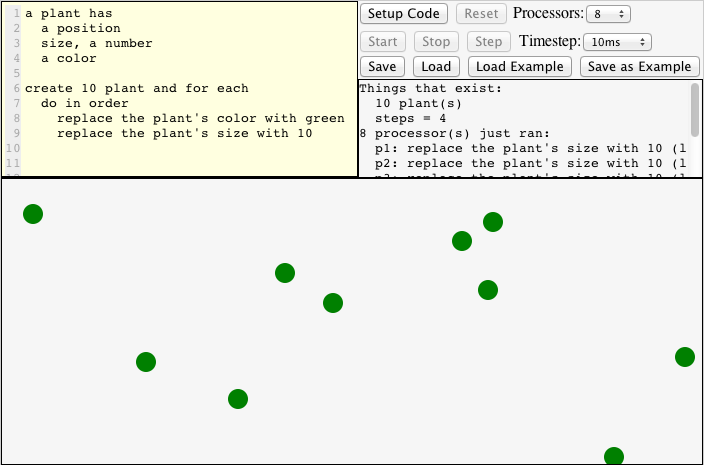
\includegraphics[width=.49\textwidth]{figures/EcosimScreencap2.png}}
\caption{The \emph{EcoSim} web-based integrated development environment hosted at
\ecosimPath{}.  Code is written and debugged in the top left window, settings are on
the top right, a console with runtime and debug information is below the settings, and the
main window shows the graphical output of the program.}
\label{fig:ecosimScreencap}
\end{figure}


\section{Background and Related Work}
% Parallelism
Parallel computing is not new, dating back to 1955 and the IBM 704~\cite{hockney1988parallel}.
However, until recently advances in individual processor speed meant single-processor machines
were sufficient for most tasks~\cite{amdahl1967validity}, 
and the bulk of programming practices and pedagogy were developed for a single-processor programming model.
Today, multicore desktop and laptop computers are ubiquitous---%
when novice programmers write their first code today, it is often running on a parallel computer.
In order to make the most efficient use of these computers, parallel programming is necessary.  


There are numerous programming languages available for desktop parallel programming.  Many of
these languages are extensions, libraries, or APIs built on top of sequential languages such 
as C or Fortran 
(e.g., OpenMP, CUDA, OpenCL, Intel Thread Building Blocks, pthreads, Cilk, Co-array Fortran, and Unified Parallel C),
requiring a novice programmer to first become proficient in a sequential language 
before tackling the parallel programming concepts.  
While this does not necessarily hinder a student's overall programming ability, 
parallel programming tends to receive less importance 
than simply learning the sequential aspects of the language.  

There are also languages designed for parallel programming, but they tend have advanced
syntax and be targeted towards
students already proficient at programming in general (e.g., X10\cite{X10}, 
NESL~\cite{nesl-impl-94}, Go~\cite{GoLanguage}, and ParaSail~\cite{ParaSail}).  It would be hard to suggest any of these
languages to an absolute beginner programmer.

% Pedagogy
Several researchers have investigated teaching parallel programming concepts 
at the undergraduate level~\cite{freshmanParallel,undergraduateParallel,gridPortal} 
and at least one at the secondary school level~\cite{highSchoolParallel}.
These studies targeted both first and second year students
using openly available parallel programming languages (e.g., OpenMP, MPI, and CUDA).
A common result was that students were motivated more by 
concrete examples of parallel code and significant classroom programming time 
rather than by abstract concepts delivered in a lecture.
We likewise utilized concrete examples and lost of in-class programming time.


% Readability
Several successful languages have been designed to have English-like syntax,
including COBOL~\cite{COBOL59}, AppleScript~\cite{AppleScript}, and Wolfram Alpha~\cite{WolframAlpha}.
Like \EcoSim{}, each was designed to accessible to non-programmers
and each targets a relatively narrow set of possible use cases.
None are targeted toward teaching parallel programming concepts.

An alternative to ``readable'' languages 
is to use a graphical rather than textual representation of the program.
Two recent examples of graphically-represented languages that are aimed at children 
are Scratch~\cite{Scratch} and Kodu~\cite{Kodu}.
While an exhaustive survey of graphical programming languages was impractical,
we were unaware of any that required no installation
and were suitable for teaching core parallel programming concepts.



\section{EcoSim: An Introductory Parallel Programming Language}
We looked for four characteristics in the language we used in our course\footnote{
We considered, but rejected, a fifth characteristic: a ``complete'' language.
As an enrichment course, we did not anticipate being a gateway into serious software development.
In hindsight, this may have been a bad choice.
}:
\begin{description}
	\item[Visibly Parallel:]
		We wanted a language that was parallel unless requested otherwise.
		We also wanted the idea of parallel processors executing the instructions
		to be emphasized throughout the language and visible in the runtime environment.
	\item[Self-Explanatory:]
		We didn't want to have to translate what code meant.
		No rebinding ``='' to be assignment instead of equality,
		no dependence on concepts past 4th-grade standards,
		and preferably no new symbols or re-defined words at all.
	\item[Web-Based:]
		We wanted the students to be able to work at home without installation.
		This meant building on top of either Javascript or Flash, 
		the only tools we could count on all the students having already installed.
	\item[Engaging:]
		We wanted every program the students wrote to interest them.
		Every program should be graphical, with text reserved for diagnostic information.
\end{description}

Since we were aware of no language having all four desired characteristics, 
we created our own.
We designed the syntax and semantics, 
wrote a type-checking parser, interpreter, and runtime environment in Javascript.
We also created an interaction environment using HTML and CSS, with the HTML5 Canvas element providing graphical output.

\subsection{The EcoSim Runtime}\label{sec:runtime}
The \EcoSim{} environment has three basic interfaces:
the code entry pane, 
a status window listing the results of parsing and the behavior of each processor,
and a graphical display of the state of each object.
The graphical display automatically draws a circle for each object
that had a defined position and size in the student's code.
By automating the display 
we were able to focus on core programming concepts
rather than teaching about a graphics API.

In addition to the user interface, the \EcoSim{} runtime provides the following:
\begin{description}
	\item[A fixed number of virtual processors.]
		At each processing step the interpreter assigns to each processor a task;
		this task is displayed both in the code pane and in the status window.
	\item[A shared work queue for ongoing tasks.]
		Processors pull jobs off this queue in a random order
		and insert any unfinished work back on the queue at the end of each step.
	\item[A global list of objects of each type.]
		Every object that is instantiated is placed on a global list of objects of that type.
		These lists are used to handle ``for each'' and ``for some'' constructs.
	\item[A collision tracker and set of collision handlers.]
		The code may provide handlers for collisions of objects with position and size.
		These are given to the processors if the work queue is empty.
	\item[A set of idle tasks.]
		If the work queue is empty and there are no collisions to handle,
		the remaining processors are given jobs from a set of low-priority tasks.
\end{description}

The runtime is aware of four types:
number (IEEE floating points), color (HTML-compliant color names), 
comparison (boolean values; used only behind the scenes to type-check guard expressions),
and position (a pair of numbers, $x$ and $y$).
User-defined types are built out of these parts.


\subsection{The EcoSim Language}
Three principles guided our design of \EcoSim{}'s language constructs:
``audience: processor'', ``self-describing syntax'', and ``anonymous by default.''
The first two are directly parallel our first two objectives:
we wanted the processors to be visible throughout the language
and the language to be self-explanatory.
We added the third principal, defaulting to anonymity,
reduced the need to come up with names for variables,
simplifying the programming process.
We hoped it would also reduce the likelihood of conflict over limited, named computing resources,
but this kind of conflict did not arise in any class example.

Rather than provide a full description of the language that grew out of these principles,
we provide here a few elements that typify language design
and rely on the language's self-describing character 
to render later code examples understandable.

\subsubsection{Statements}
The first operator we considered was the assignment operator.
We had discovered in previous interactions with CS1 students
that the syntax used in \texttt{x = x + 1} was often confusing.
We brainstormed ways we might explain that operation,
things like ``$x$ is redefined; it's new value is 1 + the old value of $x$,''
but most were too verbose or failed the ``audience: processor'' principle.
We finally settled on \code{replace x with old x + 1},
which we implemented as two rules:
an assignment syntax of \code{replace {\it lvalue} with {\it rvalue}}
and a requirement that the word \code{old} precede rvalue variables that also appear in the lvalue.

Similar processes resulted in 
\texttt{while(1<2)} becoming \code{as long as 1 $<$ 2},
\texttt{else} being replaced with \code{otherwise}, 
and \texttt{double x = 3} becoming \code{start x as 3}.
We replaced the membership operator (commonly \texttt{.} or \mbox{\texttt{->}})
with the more English-like \code{'s} (as in \code{baz's position's x}).
We also implemented type inference to create a statically-typed language 
without needing to declare variable types.

The runtime keeps a list of objects of each type (see \S\ref{sec:runtime});
we add to these lists by writing \code{create 3 number} and and remove with a \code{destroy} command.
We can access objects either by grabbing one randomly selected object:
\begin{snippet}
\STATE for some number
\INDSTATE destroy the number
\end{snippet}
or by accessing all of them in parallel:
\begin{snippet}
\STATE for each number
\INDSTATE replace the number with the old number + 1
\end{snippet}

\subsubsection{Definitions}
We observed that structures, properties, and subroutine definitions
are describing ``what we mean by $X$'' rather than ``you should do $X$''.
We thus decided that, per the ``audience: processor'' principle, 
we should word these to inform, not direct, the processor.

For example, to introduces a structure type named ``plant''
with a named field ``size'', an anonymous position field, and two anonymous colors,
we write
\begin{snippet}
\STATE a plant has
\INDSTATE size, a number
\INDSTATE a position
\INDSTATE 2 color
\end{snippet}
We can also define properties for plants:
\begin{snippet}
\STATE a plant's age is the plant's size $-$ 5
\STATE a plant's trunk is the plant's 2nd color
\end{snippet}
Properties are always single expressions and are accessed exactly like fields.
Multiple fields (such as \code{color} above) can only be accessed by compile-time ordinals like \code{5th};
you cannot write \code{the plant's $n$th color} for variable $n$.

Subroutines are defined with a ``how to'':
\begin{snippet}
\STATE how to add a number years to a plant
\INDSTATE replace the plant's size with the plant's old size + the number
\end{snippet}
Calling a subroutine is straightforward:
\begin{snippet}
\STATE for some plant
\INDSTATE add 3 years to the plant
\end{snippet}
Because this syntax for defining and calling subroutines
is context sensitive, it is not easy to achieve using most parser techniques.
Our parser type-checks and builds the symbol table as it goes,
so when we parse a line \code{how to {\it words}}
we already know which of the words identify types and which are unbound words naming the subroutine.
Similarly, we know from context that \code{the plant} is a value
and thus that we are calling a method named ``add \_\_\_ years to \_\_\_'' and not ``add \_\_\_ years to the plant''.

\subsubsection{Handlers}
The last element of the language we want to identify
is collision handlers and idle operations.
\begin{snippet}
\STATE when a bulldozer hits a plant
\INDSTATE destroy the plant
\STATE when bored
\INDSTATE create a plant
\end{snippet}
Again, these are worded to address the processor in a self-explaining way.
They prevent the need for a \texttt{main} method, since \code{when bored} will suffice,
and make event-oriented programming straightforward.
Multiple \code{when bored} declarations were permitted,
with the runtime selecting between them at random.


\section{Course Overview and Lesson Plans}
The pilot course we created was for fourth and fifth grade students in an enrichment program
that is run through our university.  We designed the course and \emph{EcoSim} concurrently,
for an audience of self-selected primary school students with no
prior formal programming experience.
%\begin{enumerate}
%\item Overview (ecosystem in parallel)
%\item Starting to "think parallel" -- student sort
%\item Ingraining the idea of multiple processors working independently to solve the same problem.
%\item Constantly let kids show off what they have accomplished
%\item the idea of "when bored", for some, for all
%\item atomicity and race conditions (class example on board -- roll/read/roll/write)
%\item St.~Matthew Island
%\end{enumerate}

\subsection{Ecosystem in Parallel}
The original conception of the pilot course was, simply, 
``Let's teach fourth and fifth graders about parallel programming.''
To streamline our lessons we decided to structure our examples around a single theme.
The theme we selected was ``ecosystems'', a topic familiar to students at that level
and one that is inherently parallel, and easy to visualize, 
and allows for a wide range of example applications.
By the end of the course students had expanded the ecosystem 
from simple static plants
to handle complex interactions between 
plants that only grew during the day and only seeded in their immediate neighborhood,
competing herbivores and hunters, carnivorous and poisonous plants,
and other more imaginative fantasy elements.

Students quickly learned the importance of initial conditions and parameters, both from a 
computational perspective and a scientific one.  For example, students found that starting 
ten thousand herbivores in a field with only ten plants
both results in over-grazing and starvation and slows the computer to a crawl.  
We spent a number of classes discussing and
modeling the intriguing real-life case of a herd of reindeer who overpopulated the remote
St.~Matthew Island in Alaska and subsequently died out~\cite{klein1968introduction,stMatthewIsland}.
With the \emph{EcoSim} model the students were able to adjust the parameters 
and look for an equilibrium that would have allowed the reindeer to survive.

\subsection{Getting the students to ``think parallel''}
We began each class period with a conversation and activity introducing a new parallel programming concept. 
For example, on the first day of class we introduced the students to the difference in
computational time between parallel and sequential processes by having them sort themselves
by height.  First, we allowed the students to line themselves up by height, all at once (the
parallel method), and we timed this; it took roughly forty-five seconds for a class of eighteen.
Next, we re-randomized the class and assigned one student to be the ``processor,'' in charge
of sorting the students two at a time.  Unsurprisingly, this took roughly twice as long, 
leading to a fruitful discussion on why parallel processing can be faster.

\begin{table*}
\centering \begin{tabular}{p{.7\linewidth} | p{.25\linewidth}} 
\toprule
Group Activity               &  Parallel Programming Concept \\ \midrule
Students sort themselves, and then one student sorts everyone.     & Parallel speedup \\ \hline
Everyone shares a pen to write on the whiteboard to increment a number. & Locks / Atomicity  \\ \hline
Students roll dice until they get a six, read a number off the board, increment it, roll more dice, and call out the new number, which is written on the board.   & Race Conditions \\ \hline
All students start with a number, and half hand to their neighbor to add together.
This continues until one student has the total sum. & Reduction and Divide/Conquer  \\
\bottomrule 
\end{tabular}
\caption{Group activities.}
\label{tab:group-activities}
\end{table*} 

Table \ref{tab:group-activities} shows the group activities we conducted and their associated
parallel processing concept or concepts.  During and after each activity, we discussed the
associated concept, and in most cases we then wrote a simple program in \emph{EcoSim} that
demonstrated the idea.  Each student sat at a computer with \emph{EcoSim} loaded into their
web browser, and they were able to type out the examples as we wrote them on the overhead 
projector.
For example, after the race condition activity, we wrote the programs in 
Figure~\ref{fig:race-conditions}, which demonstrate a race condition stemming from allowing multiple
processors to complete the \texttt{color} statements in any order.

     
\begin{figure}
\begin{algorithmic}[1]\sf
%\INDSTATE[x]{code} indents x number of tabs, \INDSTATE{code} indents a single tab
\item[{\bf In order:}]
\STATE{a moth has}
  \INDSTATE{a position}
  \INDSTATE{a color}
\STATE{a moth's size is 50}
\STATE{}
\STATE{create 10 moth and for each}
  \INDSTATE{do in order}
  \INDSTATE[2]{replace the moth's color with gray}
  \INDSTATE[2]{replace the moth's color with black}
\end{algorithmic}

\begin{algorithmic}[1]\sf
\item[{\bf In any order:}]
\STATE{a moth has}
  \INDSTATE{a position}
  \INDSTATE{a color}
\STATE{a moth's size is 50}
\STATE{}
\STATE{create 10 moth and for each}
  \INDSTATE{do in any order}
  \INDSTATE[2]{replace the moth's color with gray}
  \INDSTATE[2]{replace the moth's color with black}
\end{algorithmic} 
\caption{Example \emph{EcoSim} programs that demonstrate race conditions.  In the
``in order'' program, all moths end up black, while in the ``out of order'' program
the final color is dependent on a race condition.}
\label{fig:race-conditions} 
\end{figure}

\emph{EcoSim} allows a programmer to set the number of processors that will be used to run the
program. We used this to demonstrate a number of concepts to the students, including demonstrating
parallel speed-up and race conditions.  For example, if \emph{EcoSim} is set to use a single
processor, and the ``In order'' program from Figure~\ref{fig:race-conditions} is amended to remove
line 8, the students can see the individual ``moths'' changing color one at a time.  If we change
the simulator to run with two processors, the students can easily see that two moths change color
at a time, and with 16 processors they can see that all of the moths change all at once and the
program completes almost instantly.  With \emph{EcoSim}'s ability to step through a program, 
individual processor activity can be made even more apparent.

\subsection{The Use of Example Programs}
As with any programming course, example programs played an important role in teaching our course.
This was the first time most of the students had seen any programming language at all, and
therefore we decided to provide a scaffolding in the form of example programs that they could
look at and modify.  \emph{EcoSim} has a ``Load Example'' button that brings up a listing of
example programs that the instructors can update at any time.  Many times during class we would
have students pay attention to the projector as we typed in the code for a program, and then we
would have them load the example instead of typing it out.  This saved time (not all pre-teens
are fast typists), and it also allowed us to start the whole class at the same point in a program's
development.  In some cases we gave them example programs that were missing a line or two and
asked them to fill in the details themselves.  We encouraged the students to modify the programs
as well, and students that completed assignments before others in the class were able to modify
the example programs or load other programs they had been working on previously.

Another reason we relied on example programs was to build a compendium of programs that the students
could go back and look at if they did not remember the details of a particular topic.  Frequently,
we would direct the students to previously covered examples, and we would also keep versions of 
certain programs so they could see the steps used to create more robust programs.

\subsection{Student Assessment}
Because this was an ungraded enrichment class, we did not perform formal assessments (e.g., tests
or deadline-based homework). However, we reviewed the students' work regularly and gave feedback
often.  At the beginning of each hour of class, we asked whether anyone had something they wanted
to show the class, allowing them to display their work on the projector and describe their
programs.  This motivated the students to create interesting programs, and the students enjoyed
showing off their work to the rest of the class.  Some students showed off work that they completed
on their own at home during the week between classes, which we highly encouraged.

All student work is captured in a MySQL database that we were able to review regularly.  Each time
a student clicks on the ``Setup Code" (which parses the code and reports errors), the current
program is saved, and all versions are retained.  Therefore, we were able to look at a students 
progress, including how many attempts they made at fixing syntax errors and how they went about
writing their programs.  We used this analysis to determine where we needed to review; e.g.,
once we realized how much trouble the students had with understanding indentation and blocks, we
modified our lesson plan to include a review and further examples.

\section{Student Work and Outcomes}
During the course, the students had an opportunity to modify example programs, and they also were able to write their own applications.  
Because we had access to all modifications of each student's code, we were able to perform some
statistical analysis on their code, including determining how many different applications 
students worked on and how long it took them to fix certain coding errors.  On average, 
each student worked on twenty different programs, with some students working on as few as twelve or as many as thirty-two.  Students that worked on more programs tended to be the ones who picked up
the material the fastest, and also worked on their own at home.  The students' programs ranged 
from five-line examples to a 150-line program that 
was the culmination of the St.~Matthew Island deer/plant ecosystem simulation.
In addition, some students
created novel programs that demonstrated proficient understanding of the language.  
Figure~\ref{fig:pacmanProgram} shows part of one student's novel ``Pacman'' program, demonstrating 
an understanding of the parallel nature of the language.

\begin{figure}
\begin{algorithmic}[1]\sf
\setcounter{ALC@line}{22}
%\INDSTATE[x]{code} indents x number of tabs, \INDSTATE{code} indents a single tab
\STATE{when bored}
  \INDSTATE{for each pacman}
    \INDSTATE[2]{do in any order}
      \INDSTATE[3]{move the pacman's position a random number between 10 and 50 right}
      \INDSTATE[3]{move the pacman's position a random number between 10 and 50 left}
      \INDSTATE[3]{move the pacman's position a random number between 10 and 50 up}
      \INDSTATE[3]{move the pacman's position a random number between 10 and 50 down}
\STATE
\STATE{when a pacman hits a ghost}
  \INDSTATE{destroy the pacman}
\end{algorithmic} 
\caption{Part of one student's ``Pacman'' program, that demonstrates a competent understanding
of the programming language and its parallel programming structure.}
\label{fig:pacmanProgram} 
\end{figure}

\FIXME{Add statistics on how many tries it took students to fix parse errors.}

On the last day of class, the students had the opportunity to show off their work to their
parents and siblings. Our instruction to them on the last day was to prepare a program that
they either created on their own, or an example from class that they modified significantly.
They enthusiastically demonstrated their programs,
including various modifications to the St.~Matthew Island ecosystem,
programs that had snow ``fall'' on the screen and accumulate at the bottom,
simulations that included mice searching for cheese,
etc.

\section{Conclusions}
We have demonstrated that it is possible to teach elementary school students parallel programming,
even if they are completely novice programmers. 
We were able to teach basic programming skills as well as concepts such as race conditions, 
atomicity, locks, and the speedups that can be obtained by using multiple processors
Our experience was that none of the students had any difficulty with parallelism
and most were able to explain core parallel concepts to their parents at the end of the course.

To facilitate learning in our course, we
\begin{itemize}\itemsep=0pt \topsep=0pt
\item designed a unique, English-like parallel programming language and associated visual web interface;
\item provided a curriculum that taught programming through a parallel lens; and
\item utilized kinesthetic learning activities, think-pair-share discussions, and individual guided exploration to teach each concept.
\end{itemize}
We found the students eagerly learned the language, with few conceptual difficulties and demonstrable success.  
Parallel programming does not have to be difficult to teach or learn,
and it is a skill that will become even more important as computers continue to become more
parallel in the future.

%ACKNOWLEDGMENTS are optional
%\section{Acknowledgments}
%This section is optional; it is a location for you
%to acknowledge grants, funding, editing assistance and
%what have you.  In the present case, for example, the
%authors would like to thank Gerald Murray of ACM for
%his help in codifying this \textit{Author's Guide}
%and the \textbf{.cls} and \textbf{.tex} files that it describes.

%
% The following two commands are all you need in the
% initial runs of your .tex file to
% produce the bibliography for the citations in your paper.
%\newpage
\small{
\bibliographystyle{acm}
\bibliography{ecosim}  % sigproc.bib is the name of the Bibliography in this case
}
% You must have a proper ".bib" file
%  and remember to run:
% latex bibtex latex latex
% to resolve all references
%
% ACM needs 'a single self-contained file'!
%

\end{document}
